\documentclass[a4paper, 10pt]{exam}
\usepackage[margin=1in]{geometry}

\usepackage[utf8]{inputenc}
\usepackage{amssymb, amsmath, graphicx, multicol}
\usepackage{pgf,tikz, graphicx}
\usepackage{mdframed}
\usepackage{mathrsfs}

\everymath{\displaystyle}
\printanswers
\newmdtheoremenv{proof}{}

\begin{document}
\fbox{\textbf{Math 140 - HW 3}} 
\textbf{REGALARIO, Jeremiah Daniel A. | 2022-20670}
\begin{questions}
    \question Consider the following axioms for \textit{three-point geometry}:
    \begin{enumerate}
        \item[] \textbf{TPG1:} There are exactly three points.
        \item[] \textbf{TPG2:} Any two distinct points are on exactly one line.
        \item[] \textbf{TPG3:} Not all the points are on the same line.
        \item[] \textbf{TPG4:} Any two distinct lines are on at least one point.
    \end{enumerate}
    Demonstrate using diagrams, one for each axiom, that the axiomatic system \{TPG1, TPG2, TPG3, TPG4\} is independent. Each model must satisfy all of these three properties: 
    \begin{enumerate}
        \item[] \textbf{P1:} There is at least one but at most five points.
        \item[] \textbf{P2:}: There is at least one but at most five lines.
        \item[] \textbf{P3:} Any point is on at least one line
    \end{enumerate} \\

    \begin{enumerate}
      \item[\textbf{TPG1:}] \{$\neg$TPG1, TPG2, TPG3, TPG4\}
      \begin{proof}
            Let $\mathscr{P}(G) = \{A, B, C, D\}, \mathscr{L}(G) = \{\{A, B\},\{B, C, D\}, \{A, C\}, \{A, D\} \}$
            \begin{center}
                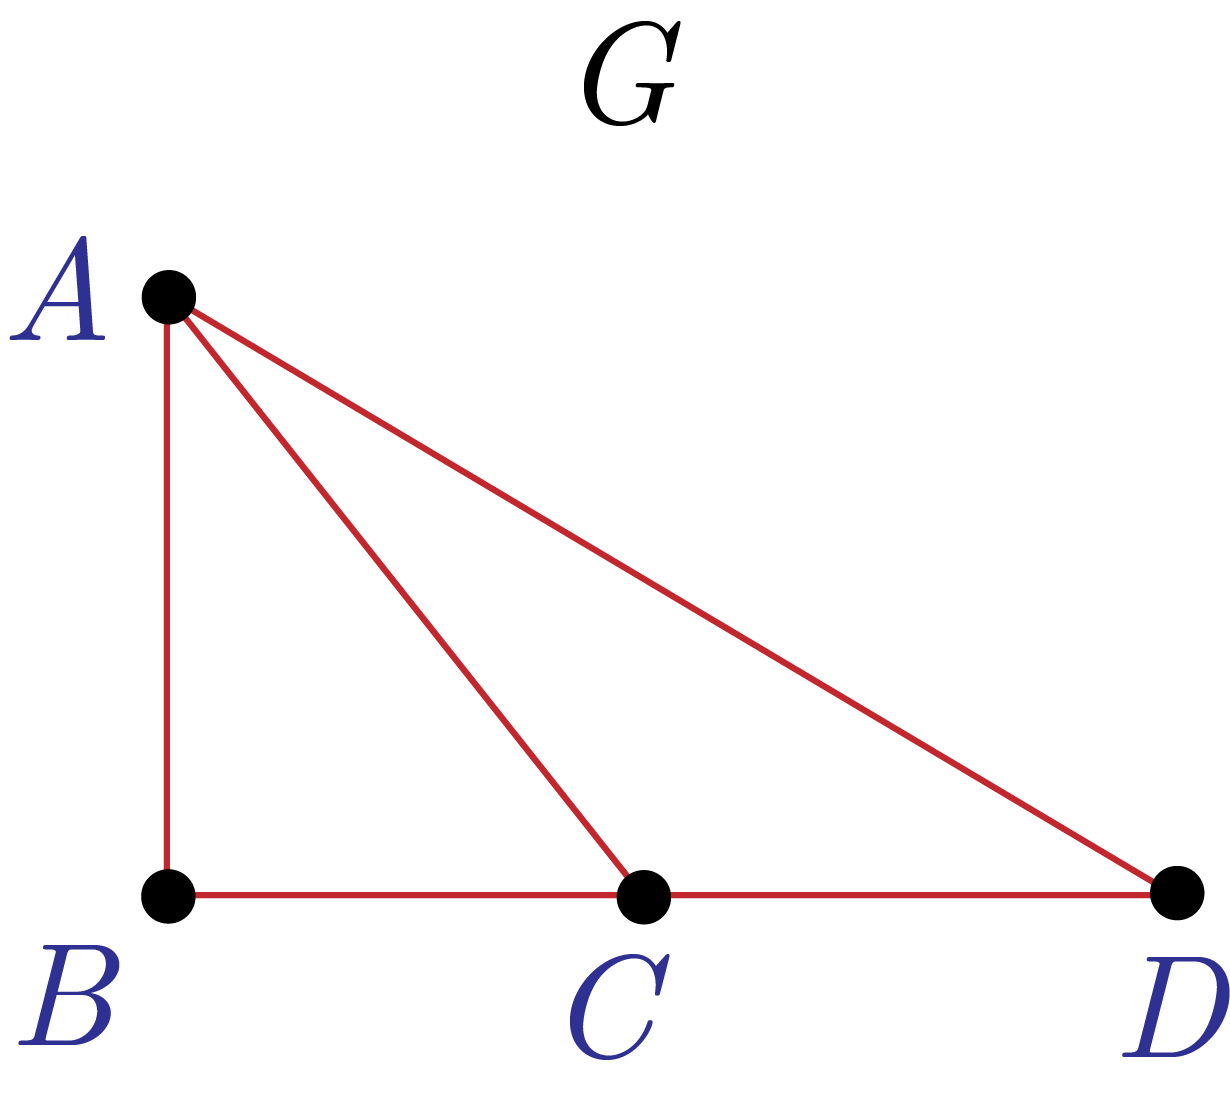
\includegraphics[width=0.3\textwidth]{3.1.png} \\
                  
            \end{center}
        \end{proof}
      \item[\textbf{TPG2:}] \{TPG1, $\neg$TPG2, TPG3, TPG4\}
      \begin{proof}
            Let $\mathscr{P}(G) = \{A, B, C\}, \mathscr{L}(G) = \{\{A, B\},\{B, C\} \}$
            \begin{center}
                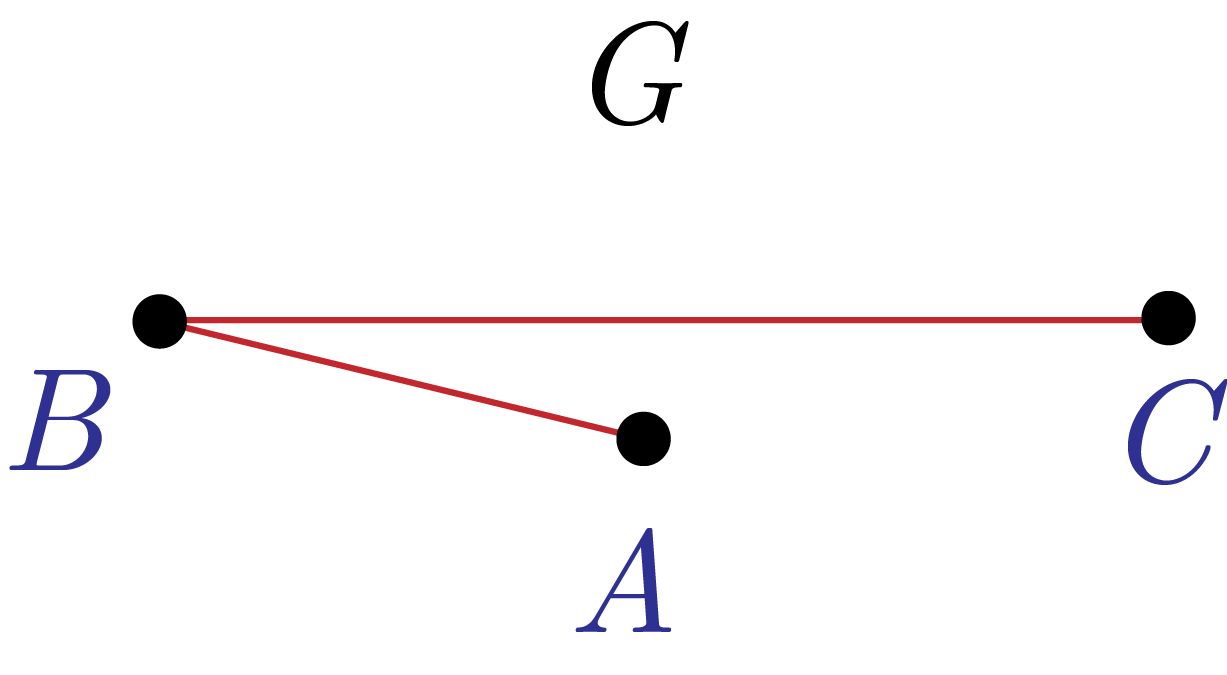
\includegraphics[width=0.3\textwidth]{3.2.png} \\
                  
            \end{center}
        \end{proof}
      \item[\textbf{TPG3:}] \{TPG1, TPG2, $\neg$TPG3, TPG4\}
      \begin{proof}
            Let $\mathscr{P}(G) = \{A, B, C\}, \mathscr{L}(G) = \{\{A, B, C\} \}$
            \begin{center}
                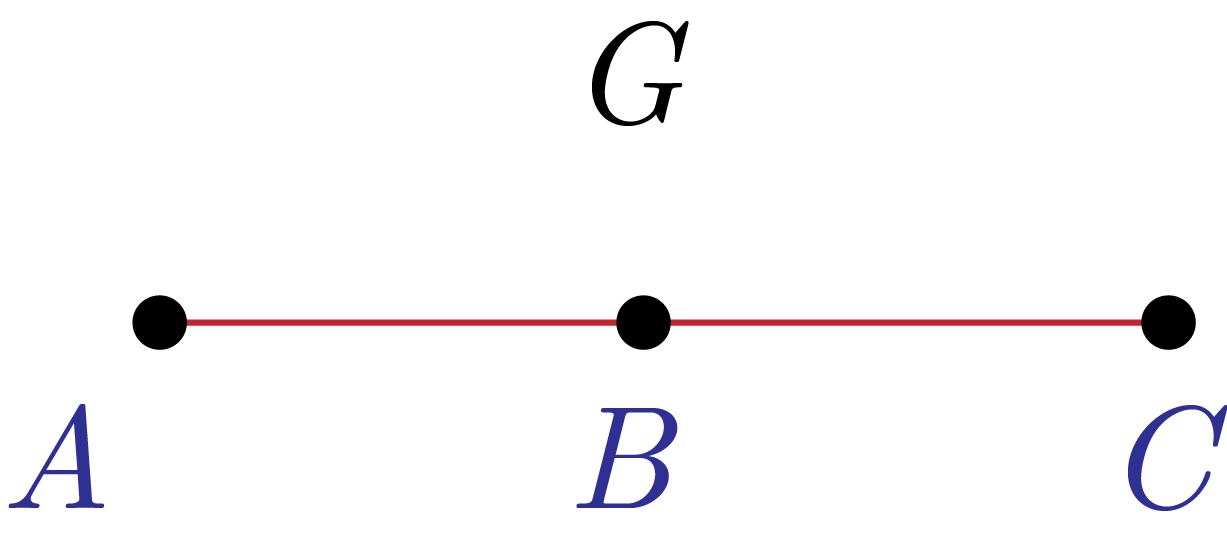
\includegraphics[width=0.3\textwidth]{3.3.png} \\
                  
            \end{center}
        \end{proof}
      \item[\textbf{TPG4:}] \{TPG1, TPG2, TPG3, $\neg$TPG4\}
      \begin{proof}
            Let $\mathscr{P}(G) = \{A, B, C\}, \mathscr{L}(G) = \{ \{A\}, \{A, B\},\{B, C\}, \{C, A\} \}$
            \begin{center}
                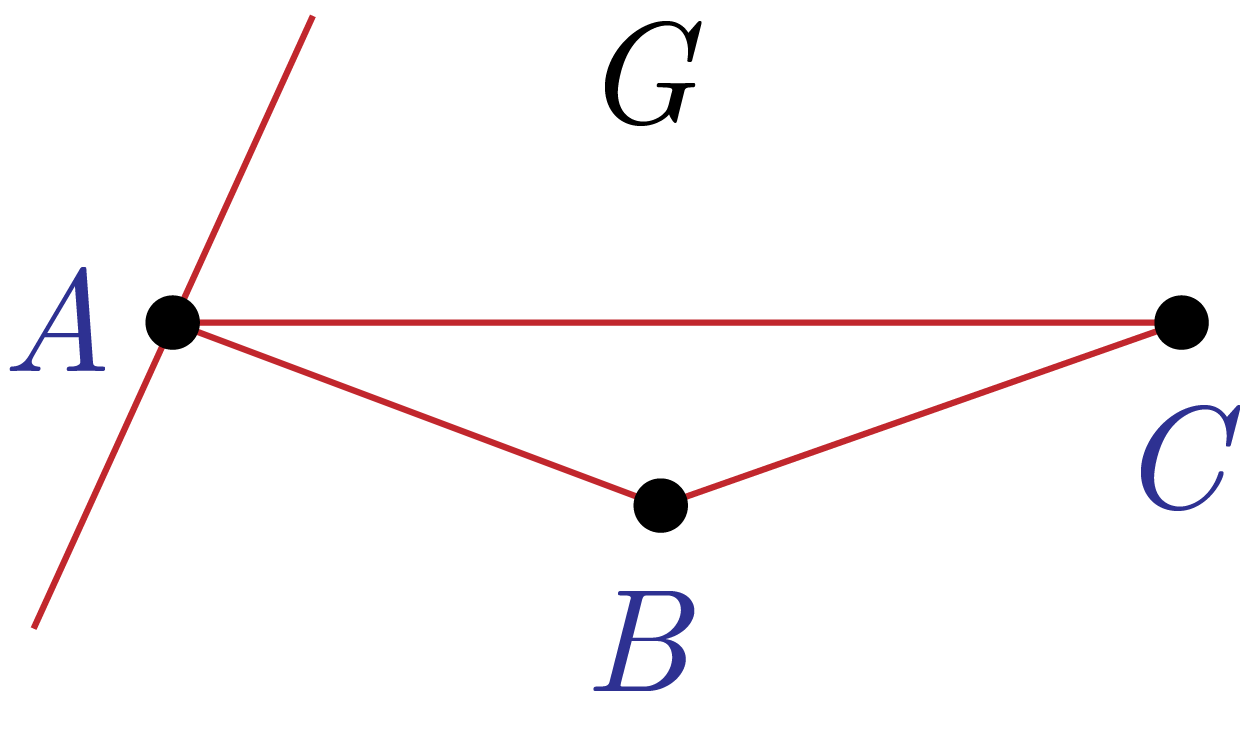
\includegraphics[width=0.29\textwidth]{3.4.png} \\
                  
            \end{center}
        \end{proof}
    \end{enumerate}

\end{questions}

\end{document}
